\section{Architektur}

In diesem Kapitel wird die derzeitige Architektur des Komponentenmodells vorgestellt. Sie setzt sich aus den in Abbildung \ref{fig:arch} dargestellten und im Folgenden kurz erl�uterten Bestandteilen zusammen. An der Umrandung der Bl�cke ist abzulesen, ob diese bereits entworfen oder lediglich als Erweiterungen geplant sind. Details und Informationen zur Umsetzung der Bestandteile des Komponentenmodells sind Inhalt der folgenden Kapitel dieses Dokuments.

\begin{figure}[ht]
 \centering 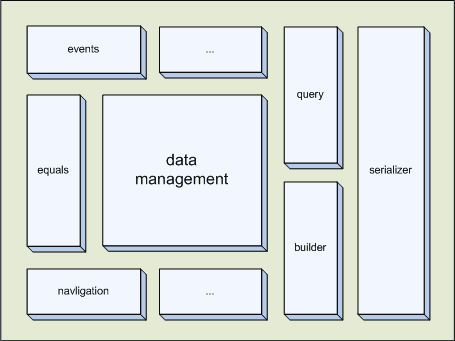
\includegraphics{arch.png}
 \caption{Architektur des Komponentenmodells}
 \label{fig:arch}
\end{figure}

Zentrum der Architektur bildet die in der Abbildung mit \emph{data management} bezeichnete Datenhaltung. Sie dient der lokalen Speicherung der Entit�ten und Relationen des Modells zur Laufzeit der nutzenden Anwendung. Hierf�r stellt sie M�glichkeiten zum Lesen und Schreiben der Daten zur Verf�gung. Die Konsistenz der Daten ist in dieser Schicht lediglich in Bezug auf die verwendeten Datenstrukturen zu gew�hrleisten. Semantische Fehler im Sinne des theoretischen Komponentenmodells sind von der Datenhaltung zu tollerieren, um unabh�ngig von m�glichen �nderungen dieser Semantik zu bleiben. Aufgrund dessen ist der das Modell nutzenden Anwendung keine M�glichkeit zu gew�hren, direkt auf die Datenhaltung zuzugreifen, da sonst Korrektheit im Sinne des theoretischen Modells nicht mehr gew�hrleistet werden kann. Zugriff ist erst nach �berpr�fung durch entsprechende Zwischenschichten zu gestatten.

Schreibende �nderungen der Anwendung am Modell sind hierbei durch den in der Architekur mit \emph{builder} bezeichneten Block vorgesehen. Dieser stellt eine Infrastruktur bereit, welche �nderungen an verschiedenen Stellen des Modells zul�sst und den korrekten Aufbau gem�� dem theoretischen Modell sicherstellt. Es k�nnen an dieser Stelle bereits durch geschickte Wahl der Zugriffsmethoden Fehler ausgeschlossen werden. Eine M�glichkeit der Umsetzung dieser Schicht unter Beachtung der Hierarchie des Komponentmodells wird in Kapitel \ref{sec:builder} vorgestellt.
  
Der lesende Zugriff auf das Modell kann je nach Bedarf durch verschiedene Schichten erfolgen. Die in Abbildung \ref{fig:arch} mit \emph{query} bezeichnete Schicht dient der Abfrage von Attributen der Entit�ten und der Beziehung zwischen diesen. Eine direkte Abfragem�glichkeit der Datenhaltung ist prinzipiell m�glich, jedoch aufgrund fehlenden Wissens �ber das theoretische Modell unpraktikabel. Abstraktionen in diesem Sinn sind also ebenfalls Aufgabe der Abfrageschicht. 